\documentclass[11pt]{article}
\usepackage{myz310e-notes}
\hypersetup{pdftitle={Risk, generalisation and model selection},pdfauthor={Emre Onur Kahya},pdfsubject={MYZ 310E Machine Learning in Physics, Fall 2026, lecture note 4 (week 2)}}

\begin{document}
\NoteTitle{4}{2}{Risk, generalisation\\ and model selection}{Risk and model selection}{%
This note turns the informal goal ``predict well on new data'' into mathematics and into a working procedure. It
defines expected and empirical risk, explains why training error is optimistic, and shows how to estimate
generalisation honestly with held-out data and cross-validation. Capacity, under- and overfitting, the
bias--variance trade-off and regularisation explain how to choose a model; the double-descent curve and scaling laws
show how deep learning has refined, without overturning, this classical picture. It is the methodological core of the
course: every later method is selected and evaluated in this way.}

\section{A learning algorithm has three ingredients}\label{sec:ingredients}

Almost every learning algorithm combines, explicitly or implicitly,
\begin{enumerate}
\item a \textbf{family of functions} $\F = \{f_\theta\}$ indexed by parameters $\theta$;
\item a \textbf{loss} $L(f(\x), y)$ that measures the cost of predicting $f(\x)$ when the truth is $y$
(Note~1, Table~2);
\item an \textbf{optimisation procedure} that searches $\F$ for a function with small average loss on the training
data.
\end{enumerate}
Families range from the trivial to the enormous: constant predictors $f(\x) = b$; affine functions
$f(\x) = \vect{w}\T\x + b$; polynomials of degree $p$; the piecewise-constant functions of histograms (Note~3);
weighted sums of kernels centred on the data (Note~5); decision trees; neural networks, where each architecture
defines a different family. Choosing the family is the most consequential decision in a project, and it is the
subject of this note.

\section{Measuring quality}\label{sec:quality}

What we ultimately care about is rarely the loss the algorithm minimises. A hierarchy of measures is common:
\begin{enumerate}
\item the real objective in the full system --- lives saved, money earned, the statistical significance of a
physics measurement;
\item a field-specific metric --- BLEU for translation, area under the ROC curve for a trigger, word error rate for
speech;
\item a generic metric --- classification error, precision and recall, mean squared error;
\item the training loss actually optimised.
\end{enumerate}
The lower levels are proxies for the higher ones, and the gap between them deserves attention.

\paragraph{Surrogate losses} The classification error $\ind{f(\x) \ne y}$ is piecewise constant in the parameters,
so its gradient is zero almost everywhere, and even for linear classifiers minimising it exactly is computationally
hard. One therefore trains a real-valued score and minimises a smooth \emph{surrogate} that upper-bounds or tracks
the error:

\begin{center}\small
\begin{tabular}{@{}L{0.27\linewidth}L{0.37\linewidth}L{0.28\linewidth}@{}}
\toprule
Model output & Surrogate loss & Decision rule \\
\midrule
$g(\x) \approx P(Y = 1 \mid \x)$ & binary cross-entropy $-y\log g - (1-y)\log(1-g)$ & $f(\x) = \ind{g(\x) > \tfrac12}$ \\
$\vect{g}(\x) \approx (P(Y = k \mid \x))_{k}$ & cross-entropy $-\log g_y(\x)$ & $f(\x) = \argmax_k g_k(\x)$ \\
score $g(\x)$, $t = 2y - 1 \in \{\pm1\}$ & hinge $\max(0,\, 1 - t\,g(\x))$ & $f(\x) = \ind{g(\x) > 0}$ \\
scores $g_1(\x), \dots, g_m(\x)$ & margin $\max\big(0,\, 1 + \max_{k \ne y} g_k - g_y\big)$ & $f(\x) = \argmax_k g_k(\x)$ \\
\bottomrule
\end{tabular}
\end{center}

The cross-entropies are negative log-likelihoods of a categorical model (Note~2, Section~2); the hinge and margin
losses are used by support vector machines. Probabilistic outputs have an extra benefit: the threshold can be moved
after training to trade one kind of error for another.

\begin{physics}{efficiency, rejection and the ROC curve}
A trigger or tagger outputs a score $g(\x)$, and the analysis keeps events with $g(\x) > c$. Lowering $c$ raises
the signal efficiency and lowers the background rejection; the curve traced by all thresholds is the ROC curve. The
best threshold is fixed by the physics goal --- for instance, the expected discovery significance --- not by the
training loss, which is why classifiers in physics are trained with cross-entropy and then evaluated on the full ROC
curve.
\end{physics}

\begin{modern}{training loss versus what we want}
Language models are pre-trained to minimise next-token cross-entropy, yet they are judged on answering questions,
writing code and following instructions. Closing that gap is the purpose of fine-tuning on human preferences, in which
a second model is trained to predict which of two answers people prefer and the language model is then optimised for
that learned reward. The hierarchy above, with level~4 refined step by step towards level~1, is a large part of how
current assistants are built.
\end{modern}

\section{Expected risk and empirical risk}\label{sec:risk}

Assume, as in Note~1, that examples are i.i.d.\ draws from an unknown $P(\X, Y)$. The \emph{expected risk}
(generalisation error) of a fixed predictor $f$ is its average loss on future data,
\[
  \Risk(f) = \E_{(\X, Y) \sim P}\big[L(f(\X), Y)\big],
\]
and its \emph{empirical risk} on a finite set $D$ is
\[
  \ERisk(f, D) = \frac{1}{|D|}\sum_{(\x, y) \in D} L(f(\x), y).
\]
We cannot compute $\Risk(f)$, because $P$ is unknown, but if $f$ was chosen \emph{without using} $D$, then
$\ERisk(f, D)$ is an average of i.i.d.\ terms with mean $\Risk(f)$: it is unbiased and converges to $\Risk(f)$ as
$|D| \to \infty$. Its precision follows from the variance of an average. For the classification error $p$ estimated on
$n_{\mathrm{test}}$ examples the standard error is $\sqrt{p(1-p)/n_{\mathrm{test}}}$; with $p = 10\%$ and $1000$ test
examples that is about $\pm 0.95$ percentage points. Differences between models smaller than this are not evidence of
anything.

\paragraph{Empirical risk minimisation} Since the expected risk is out of reach, learning minimises its estimate on
the training set,
\[
  \hat f = \argmin_{f \in \F} \ERisk(f, \Dtrain).
\]
This is the training phase. But now $\hat f$ \emph{was} chosen using $\Dtrain$, specifically to make
$\ERisk(\hat f, \Dtrain)$ small, so the training error is biased downwards as an estimate of $\Risk(\hat f)$ --- often
drastically, as the histogram classifier of Note~3 showed (5.2\% training error, 34.6\% test error).

\begin{keyidea}[Never evaluate on data used for choosing]
$\ERisk(f, D)$ is an honest estimate of $\Risk(f)$ only if $D$ played no part in choosing $f$ --- not in fitting the
parameters, not in choosing hyperparameters, not in pre-processing, not in deciding which model to report.
\end{keyidea}

\section{Estimating generalisation}\label{sec:estimating}

\paragraph{Hold-out} Shuffle the data and split it: train on one part, report the empirical risk on the other. This
is simple and correct, but with little data it wastes examples and gives a noisy estimate.

\paragraph{$k$-fold cross-validation} Split the data into $k$ blocks of roughly equal size. For $j = 1, \dots, k$,
train on all blocks except $j$ and compute the loss on block $j$; average the $k$ results. Every example is used once
for evaluation and $k-1$ times for training. Typical values are $k = 5$ or $10$; $k = n$ is
\emph{leave-one-out}. Cross-validation estimates the performance of the \emph{procedure} trained on a fraction
$(k-1)/k$ of the data, not of one particular fitted function.

\paragraph{Splits that respect the structure of the data} Shuffling assumes i.i.d.\ examples. When that fails
(Note~1, Section~2), the split must follow the dependence:
\begin{itemize}
\item \emph{Groups}: all measurements of the same galaxy, patient, sample or detector run go into the same block, or
the model is tested on objects it has already seen.
\item \emph{Time}: for forecasting, train on the past and validate on the block that follows, then roll the window
forward (sequential validation). A random split would let the model learn from the future.
\item \emph{Simulation and reality}: a model trained and validated on simulation must still be tested on real data,
or on a control region of it, before its performance is believed.
\end{itemize}

\paragraph{Nested cross-validation} When the same small dataset must both select hyperparameters and estimate the
error of the whole procedure, use two loops: an outer cross-validation for the estimate and, inside each outer
training set, an inner cross-validation for the selection.

\section{Capacity, underfitting and overfitting}\label{sec:capacity}

The \emph{capacity} of a family $\F$ is, informally, how many different patterns it can fit. It usually grows with the
number of free parameters, but what matters is the effective number of degrees of freedom: constraints, shared
parameters or regularisation can make a large model behave like a small one. For restricted settings capacity can be
measured exactly; for example, the Vapnik--Chervonenkis dimension of affine classifiers in $\R^d$ is $d + 1$, the
largest number of points they can label in every possible way.

Figure~\ref{fig:polyfits} shows the three regimes on $15$ noisy points from $\sin(\pi x)$. A straight line cannot follow
the curve (\emph{underfitting}: high training and test error). A polynomial of degree~$12$ passes close to every point and
oscillates wildly between them (\emph{overfitting}: low training error, high test error). Degree~$3$ captures the trend
and ignores the noise.

\begin{figure}[h]
\centering
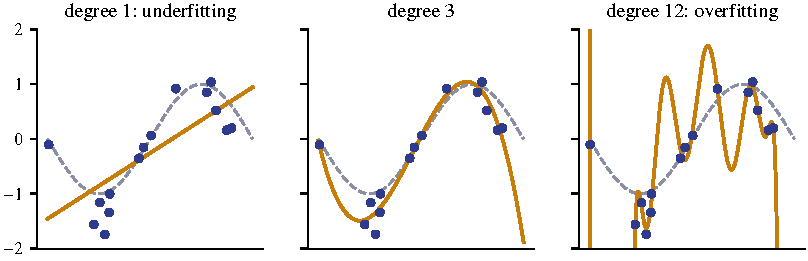
\includegraphics[width=\linewidth]{figures/poly_fits.pdf}
\caption{Least-squares polynomial fits to the same 15 points (dashed: the true function $\sin(\pi x)$).}
\label{fig:polyfits}
\end{figure}

Averaging over many training sets gives Figure~\ref{fig:capacity}: training error decreases monotonically with the
degree, while validation error first falls, reaches its minimum at degree~3 and then rises steeply. The optimal
capacity depends on the amount of data --- with more points, higher degrees become affordable. Occam's razor, ``prefer
the simplest model that explains the data'', is the qualitative version of this curve.

\begin{figure}[h]
\centering
\begin{minipage}[t]{0.49\linewidth}\centering
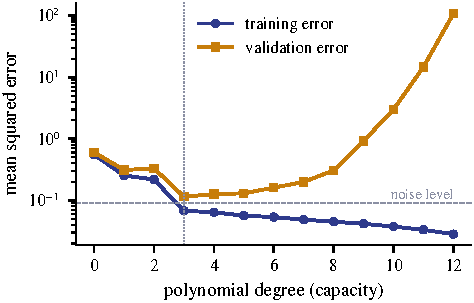
\includegraphics[width=\linewidth]{figures/capacity_curve.pdf}
\caption{Median training and validation error over 200 training sets of $n = 20$ points. The dashed line is the noise
variance $0.09$, the smallest error any predictor can achieve.}
\label{fig:capacity}
\end{minipage}\hfill
\begin{minipage}[t]{0.49\linewidth}\centering
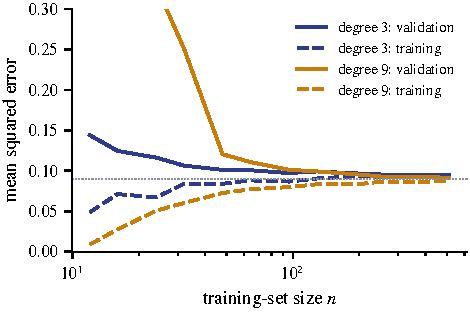
\includegraphics[width=\linewidth]{figures/learning_curve.pdf}
\caption{Learning curves: median error against training-set size for degrees~3 and~9. Training and validation error
converge to the same limit; the more flexible model needs more data to get there.}
\label{fig:learningcurve}
\end{minipage}
\end{figure}

\section{Where the error comes from}\label{sec:decomposition}

Let $f^* = \argmin_f \Risk(f)$ be the best possible predictor (its risk is the Bayes risk of Note~1, Section~4),
$f_{\F} = \argmin_{f \in \F} \Risk(f)$ the best member of the family, and $\hat f$ the function returned by the
algorithm. Then
\[
  \Risk(\hat f) - \Risk(f^*) = \underbrace{\Risk(f_{\F}) - \Risk(f^*)}_{\text{approximation error}}
  + \underbrace{\Risk(\hat f) - \Risk(f_{\F})}_{\text{estimation error}} .
\]
The approximation error shrinks as $\F$ grows; the estimation error --- the price of having to find $f_{\F}$ from
finitely many noisy examples --- grows with the size of $\F$ and shrinks with $n$.

\paragraph{Bias and variance for squared loss} Let $y = f^*(\x) + \varepsilon$ with $\E[\varepsilon] = 0$ and
$\Var(\varepsilon) = \sigma^2$, and let $\hat f_D$ be trained on a random training set $D$. At a fixed $\x$, averaging
over both $D$ and the noise,
\begin{equation}\label{eq:biasvar}
  \E\big[(y - \hat f_D(\x))^2\big] = \underbrace{\sigma^2}_{\text{noise}}
  + \underbrace{\big(f^*(\x) - \E_D[\hat f_D(\x)]\big)^2}_{\text{bias}^2}
  + \underbrace{\Var_D\big(\hat f_D(\x)\big)}_{\text{variance}} .
\end{equation}
Bias measures how far the \emph{average} fitted function is from the truth; variance measures how much the fit
changes from one training set to another. A richer family lowers bias and raises variance; more data lowers variance
(Figure~\ref{fig:learningcurve}), which is why ``the best regulariser is more data''. The proof extends the
decomposition of Note~1, Section~4, by one line (Exercise~E2).

\section{Model selection}\label{sec:selection}

\paragraph{Parameters and hyperparameters} \emph{Parameters} are fitted by the training algorithm;
\emph{hyperparameters} are fixed before training and control the family, the preference among its members or the
optimisation. They usually control capacity, which is why they cannot be chosen on the training set: the training
error would always favour the largest capacity.

\begin{center}\small
\begin{tabular}{@{}L{0.22\linewidth}L{0.38\linewidth}L{0.32\linewidth}@{}}
\toprule
Method & Hyperparameters & Parameters \\
\midrule
Histogram (Note~3) & number and placement of bins & counts in each cell \\
$k$-NN (Note~5) & $k$, the distance & none beyond the stored training set \\
Parzen windows (Note~5) & kernel and its width & none beyond the stored training set \\
Polynomial regression & degree, regularisation strength $\lambda$ & coefficients \\
Neural network & architecture, learning rate, batch size, training time, $\lambda$ & weights and biases \\
\bottomrule
\end{tabular}
\end{center}

\begin{algorithm}[h]
\caption{Model selection with a training, a validation and a test set}
\label{alg:selection}
\begin{algorithmic}[1]
\State Shuffle (or split by group or time, Section~\ref{sec:estimating}) and divide $D$ into $\Dtrain$, $\Dvalid$, $\Dtest$
\For{each candidate algorithm $A$ and each hyperparameter setting $\lambda$}
  \State $\hat f_{A,\lambda} \gets A_\lambda(\Dtrain)$ \Comment{fit parameters}
  \State $e_{A,\lambda} \gets \ERisk(\hat f_{A,\lambda}, \Dvalid)$ \Comment{out-of-sample score}
\EndFor
\State $(A^*, \lambda^*) \gets \argmin e_{A,\lambda}$
\State Optionally refit: $f^* \gets A^*_{\lambda^*}(\Dtrain \cup \Dvalid)$
\State \Return $f^*$ and the estimate $\ERisk(f^*, \Dtest)$ \Comment{$\Dtest$ used once, at the very end}
\end{algorithmic}
\end{algorithm}

The validation error of the winner is itself optimistic --- it was the minimum over many candidates --- which is why
a separate test set is needed. Cross-validation can replace the single validation set in line~4. For more than two
or three hyperparameters a grid becomes expensive; random search covers the important directions far more
efficiently, because usually only a few hyperparameters matter~\cite{bergstra2012}.

\paragraph{Regularisation} Instead of choosing among nested families, one can keep a rich family and add a
preference for simple members,
\[
  \hat f_\lambda = \argmin_{f \in \F} \; \ERisk(f, \Dtrain) + \lambda\, \Omega(f),
\]
where $\Omega$ penalises complexity and $\lambda \ge 0$ is a hyperparameter. Weight decay ($\Omega = \norm{\vect{w}}^2$)
is the most common choice; stopping the optimisation early, injecting noise (dropout) and augmenting the data with
transformed copies act as implicit regularisers. Shrinking the covariance estimate in Note~2 is the same idea.

\begin{physics}{blind analysis}
Particle and nuclear physicists guard against tuning an analysis towards the answer they expect by \emph{blinding}:
the signal region, or the final numerical result, stays hidden while selection criteria and corrections are fixed
on simulation and control regions, and is revealed only once~\cite{klein2005}. This is Algorithm~\ref{alg:selection}
with the test set locked in a drawer --- the discipline that keeps $\ERisk(f^*, \Dtest)$ honest.
\end{physics}

\begin{modern}{test sets wear out}
Benchmarks are reused by thousands of papers, so the test set slowly becomes a validation set. When ImageNet's test set
was re-created by following the original collection process, accuracies dropped by 11--14 percentage points, although
the ranking of models was largely preserved~\cite{recht2019}. For language models trained on much of the public web, a
second danger is \emph{contamination}: benchmark questions and their answers may be in the training data. Fresh,
private or time-stamped test sets are the remedy.
\end{modern}

\section{Beyond the U-shaped curve}\label{sec:modern}

Modern neural networks often have far more parameters than training examples and can fit even randomly labelled
data~\cite{zhang2017}, yet they generalise well. Figure~\ref{fig:doubledescent} shows a simple model with the same behaviour: least
squares on $p$ random nonlinear features of $n = 100$ training points. As $p$ grows the test error first follows the
classical U, then rises sharply as $p$ approaches $n$ --- where the model can just interpolate the data and the fit is
extremely sensitive to noise --- and then \emph{decreases again}. Beyond $p = n$ there are infinitely many interpolating
solutions, and the algorithm returns the one of smallest norm; as $p$ grows, that implicit preference makes the fit
smoother. In this example the test error at $p = 6000$ (0.134) is below the best value of the classical regime
(0.141).

\begin{figure}[h]
\centering
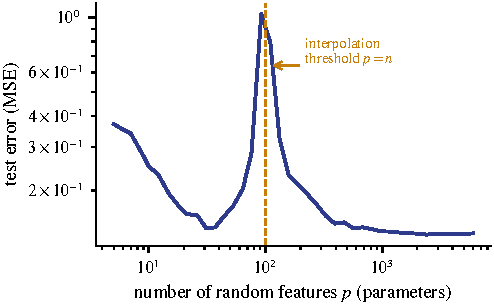
\includegraphics[width=0.56\linewidth]{figures/double_descent.pdf}
\caption{Double descent: median test error of minimum-norm least squares on $p$ random ReLU features of
10-dimensional inputs, $n = 100$ training points, 20 repetitions.}
\label{fig:doubledescent}
\end{figure}

This \emph{double descent}~\cite{belkin2019,nakkiran2020} does not overturn the ideas of this note; it refines what
``capacity'' means. The number of parameters is a poor measure of it; the norm of the solution, set implicitly by the
optimiser, matters more. Validation still decides. The other modern lesson concerns scale: for language models, test
loss falls as a smooth power law in model size, data and compute over many orders of
magnitude~\cite{kaplan2020}, and for a fixed compute budget model size and number of training tokens should grow
together, at roughly twenty tokens per parameter~\cite{hoffmann2022}. Learning curves like
Figure~\ref{fig:learningcurve}, measured on small models, are now used to plan the training of large ones.

\begin{keyidea}[Summary]
A learning algorithm is a family, a loss and an optimiser. Training minimises empirical risk, which underestimates the
expected risk of the result; honest estimates need data never used for any choice, via hold-out or cross-validation,
with splits that respect groups and time. Capacity trades approximation against estimation error (bias against
variance); hyperparameters and regularisation control it and are chosen on validation data, with the test set used
once. Over-parameterised models add a second descent of the test error, but not a new principle.
\end{keyidea}

\begin{exercises}
\item A classifier has 8.0\% error on a test set of 500 examples and another has 7.0\%. Estimate the standard error of
each. Are the two classifiers distinguishable? How large a test set would make a one-point difference significant at
about two standard errors?
\item Prove \eqref{eq:biasvar}. Start from Note~1's decomposition at fixed $\x$ and add and subtract
$\E_D[\hat f_D(\x)]$.
\item Explain why choosing $k$ for $k$-NN by minimising the training error always gives $k = 1$, and what the
training error of $1$-NN is.
\item Ten research groups each try 20 hyperparameter settings on the same public validation set and report the best.
Why is the reported number optimistic? Simulate this with a classifier that guesses at random on a balanced binary
problem with 200 validation examples.
\item Reproduce Figure~\ref{fig:capacity} for $n = 20$, $100$ and $1000$ and report the degree that minimises the
validation error in each case. Then fix degree~$12$ and $n = 20$ and add weight decay; plot validation error against
$\lambda$.
\item Galaxy images come from 300 telescope pointings, several galaxies per pointing. Design the cross-validation
splits, and explain what a naive random split would overestimate.
\end{exercises}

\paragraph{Further reading} Hastie, Tibshirani and Friedman~\cite{hastie2009}, chapter~7; Murphy~\cite{murphy2022},
chapters~4--5; for double descent, Belkin \emph{et al.}~\cite{belkin2019}.

\begin{thebibliography}{99}\small
\bibitem{belkin2019} M.~Belkin, D.~Hsu, S.~Ma and S.~Mandal, Reconciling modern machine-learning practice and the classical bias--variance trade-off, \emph{Proc.\ Natl.\ Acad.\ Sci.\ USA} 116, 15849--15854 (2019).
\bibitem{bergstra2012} J.~Bergstra and Y.~Bengio, Random search for hyper-parameter optimization, \emph{J.\ Mach.\ Learn.\ Res.}\ 13, 281--305 (2012).
\bibitem{hastie2009} T.~Hastie, R.~Tibshirani and J.~Friedman, \emph{The Elements of Statistical Learning}, 2nd ed., Springer (2009).
\bibitem{hoffmann2022} J.~Hoffmann \emph{et al.}, Training compute-optimal large language models, \emph{NeurIPS} (2022).
\bibitem{kaplan2020} J.~Kaplan \emph{et al.}, Scaling laws for neural language models, arXiv:2001.08361 (2020).
\bibitem{klein2005} J.~R. Klein and A.~Roodman, Blind analysis in nuclear and particle physics, \emph{Annu.\ Rev.\ Nucl.\ Part.\ Sci.}\ 55, 141--163 (2005).
\bibitem{murphy2022} K.~P. Murphy, \emph{Probabilistic Machine Learning: An Introduction}, MIT Press (2022).
\bibitem{nakkiran2020} P.~Nakkiran \emph{et al.}, Deep double descent: where bigger models and more data hurt, \emph{ICLR} (2020).
\bibitem{recht2019} B.~Recht, R.~Roelofs, L.~Schmidt and V.~Shankar, Do ImageNet classifiers generalize to ImageNet?, \emph{ICML} (2019).
\bibitem{zhang2017} C.~Zhang, S.~Bengio, M.~Hardt, B.~Recht and O.~Vinyals, Understanding deep learning requires rethinking generalization, \emph{ICLR} (2017).
\end{thebibliography}

\SourceNote
\end{document}
